\chapter{Mappe conformi}

Una conseguenza delle equazioni di Cauchy-Riemann soddisfatte dalle componenti
reali di una funzione olomorfa è 

\begin{corollary}
  La matrice Jacobiana della funzione reale $\morphism{(u,v)}{\Omega \subset
  \R^2}{\R^2}$ è
  \begin{equation*}
    J_f = \left(\begin{array}{cc} 
        u_x & -v_x\\
        v_x & u_x
    \end{array}\right) 
  \end{equation*}
  se inoltre $\morphism{f}{\C}{\C}$ e tale che $f = u + iv$ è una funzione
  olomorfa allora vale che
  \begin{equation*}
    \det J_f = u^2_x + v^2_x = |f'(z)|^2 \ge 0 
  \end{equation*}
\end{corollary}

\begin{remark}
  La proprietà descritta nel Corollario precedente descrive mappe che hanno un 
  senso geometrico molto importante. Infatti se $f'(z_0) \neq 0$, vuol dire che
  la mappa preserva gli angoli. Se vale questa proprietà, si dice che una mappa
  è \textbf{conforme} in $z_0$.
  \label{rmk:conforme_intuizione}
\end{remark}

\begin{theorem}
 \label{thr:conferme_sse_jacobiana_non_nulla}
  Sia $\morphism{f}{\Omega}{\C}$ e $z_0 \in \Omega$. Sia $f = u + iv$ con $u,v$
  differenziabili in $z_0$. Allora $f$ è conforme in $z_0$ se e solo se esiste
  la derivata complessa di $f'(z_0)$ e vale che $f'(z_0) \neq 0$.
\end{theorem}
\begin{proof}\
  \begin{enumerate}
    \item[$\Rightarrow$] Se $f$ è differenziabile in $z_0$ allora $J_f(z_0) = 
      |f'(z_0)|^2 > 0$ per ipotesi. Sia quindi $(u_x,v_x) = (r\cos\theta, 
      r\sin\theta)$ con 
      \begin{equation*}
        r = \sqrt{u_x^2 + v_x^2} = |f'(z_0)|^2 > 0 
      \end{equation*}
      allora la matrice Jacobiana di $f$ in $z_0$ diventa
      \begin{equation*}
        \left(\begin{array}{cc}
          r & 0 \\
          0 & r
      \end{array}\right)
       \left( \begin{array}{cc}
          \cos\theta & - \sin \theta \\
          \sin \theta & \cos \theta
      \end{array}\right)
      \end{equation*}
      corrisponde alla composizione di una rotazione con una omotetia, ma sono
      entrambe trasformazioni che preservano gli angoli, da cui la tesi.
    \item[$\Leftarrow$] Sia $f$ conforme in $z_0$. Sia $\theta$ l'angolo tra
      i vettori $(1,0)$ e $J(1,0)$ con $J = J_f(z_0)$. Per cui costruiamo una
      rotazione $R_\theta$ tale che $R_\theta^{-1}(J(1,0)) = (r,0)$ con $r > 0$
      dato che se no $f$ non preserverebbe gli angoli. In particolare chiediamo
      $R^{-1}_\theta$ una rotazione che rende l'angolo tra $(1,0)$
      e $R^{-1}_\theta(J(1,0))$ sia nullo. Segue che la
      trasformazione $G = R^{-1}_\theta J$ preserva gli angoli. Quindi segue che
      anche $G (0,1) = (0, s)$ con $s > 0$.  Per cui $G(1,1) = (r,s)$
      e dev'essere che $r = s$ dato che se non preserverebbe gli angoli. Per cui
      consideriamo $(a,b)$ vettore qualsiasi, vale che $G(a,b) = r(a,b)$.
      Because algebra: 
      \begin{equation*}
        R^{-1}_\theta J = I_r \Longrightarrow J = J_f(z_0) = R_\theta I_r
      \end{equation*}
      scritto in termini matriciali diventa
      \begin{equation*}
        J_f(z_0) = \left( 
          \begin{array}{cc}
          u_x & u_y \\
          v_x & v_y 
          \end{array}\right) = 
          \left( 
            \begin{array}{cc}
              r\cos\theta & -r\sin\theta \\
              r\sin\theta & r\cos\theta 
            \end{array}
          \right)
      \end{equation*}
      da cui segue subito che $u_x = v_y$ e $u_y = - v_x$, ovvero soddisfa le
      condizioni di Cauchy-Riemann. Pertanto $f$ è differenziabile e inoltre
      vale che $f'(z_0) \neq 0$ dato che $J \neq 0$.
  \end{enumerate}
\end{proof}

\begin{corollary}
  Una funzione $f$ complessa è conforme in $\Omega$ se e solo se $f \in
  \mathcal{O}(\Omega)$ e $f'(z) \neq 0$ per ogni $z \in \Omega$. 
  \label{cor:estensione_teorema_conformita}
\end{corollary}

\begin{definition}
  Si dice che $\morphism{g}{\Omega}{\C}$ è una funzione \textbf{antiolomorfa} se
  esiste $\morphism{f}{\Omega}{\C}$ funzione olomorfa su $\Omega$ tale che
  $\overline{g} = f$.
  \label{def:antiolomorfa}
\end{definition}

\begin{remark}
  Se si richiede che $f$ conservi solo l'ampiezza dell'angolo e non
  l'orientazione, allora anche le funzioni antiolomorfe giocano un ruolo.
  Infatti se una funzione $g$ è antiolomorfa si ha che $J_g \le 0$ e chiedendo
  che $J_g \neq 0$ si ottiene una mappa che non modifica l'ampiezza degli
  angoli, ma ne inverte l'orientazione.  
  \label{rmk:anticonformita}
\end{remark}

\begin{remark}
  La mappa $f$ è conforme in $z_0$ se e solo se per ogni coppia di vettori non
  nulli $a,b \in \R^2$, l'angolo in $z_0$ tra due curve $\gamma_a, \gamma_b$ con
  $\gamma_a(0) = \gamma_b(0) = z_0$ e $\gamma'_(0) = a$, $\gamma'_b(0) = b$
  è uguale all'angolo in $f(z_0)$ e le curve $f \circ \gamma_a, f \circ
  \gamma_b$. \\

  \begin{figure}[h]
    \centering
    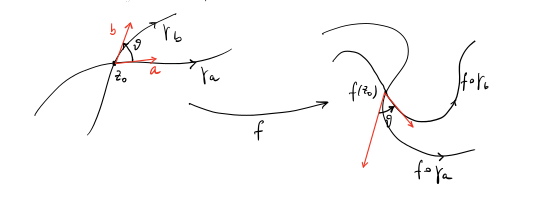
\includegraphics[width=0.6\linewidth]{images/analisi_complessa/es_mappa_conforme1.png}
    \caption{Rappresentazione della condizione di mantenimento dell'angolo tra
    due curve}
    \label{fig:mappe_conformi_1}
  \end{figure}

  Infatti se $f = u+iv$ e $\gamma_a(t) = (x(t), y(t))$, si ha 
  \begin{equation*}
    (f\circ \gamma_a)' = (u_x x' + u_y y') + i(v_x x' + v_y y')
  \end{equation*}
  e quindi vale 
  \begin{equation}
    \label{eq:globglob}
    (f\circ \gamma_a)'(0) = \left(\begin{array}{cc}
        u_x & u_y \\
        v_x & v_y 
    \end{array}\right) 
        \left(\begin{array}{c}
            x'(0) \\
            y'(0) 
        \end{array}\right) = J_f(z_0)a
  \end{equation}
  $(f\circ \gamma_a)'(0) = J_f(z_0) a$ e analogamente vale
  $(f\circ \gamma_b)'(0) = J_f(z_0) b$. Per cui dato che l'angolo viene 
  preservato, segue che $J_f(z_0) > 0$ e $f$ risulta essere conforme in $z_0$.\\

  Analogamente se $f$ è conforme abbiamo che $J_f(z_0) \neq 0$ e vale comunque
  l'identità \eqref{eq:globglob}, da cui si ha che 
  \begin{align*}
    \gamma'_a(0) = a & \parallel (f \circ \gamma_a)'(0) = J_f(z_0) a\\
    \gamma'_b(0) = b & \parallel (f \circ \gamma_b)'(0) = J_f(z_0) b
  \end{align*}
\end{remark}

\begin{example}\
  \begin{enumerate}
    \item Sia $f(z) = z^2$ allora possiamo osservare che $f'(z) \neq 0$ per $z
      \neq 0$. Quindi $f$ risulta essere conforme in $\C \setminus \left\{ 0
      \right\}$.
      \begin{figure}[h]
        \centering
        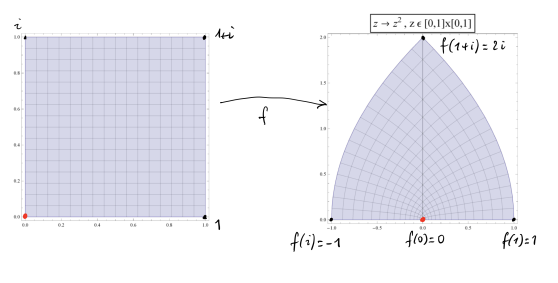
\includegraphics[width=0.6\linewidth]{images/analisi_complessa/es_mappa_conforme2.png}
        \caption{Visualizzazione di come vengono mantenuti gli angoli al di
        fuori del punto $0$}
        \label{fig:mappe_conformi_esempio1}
      \end{figure}
    \item Sia $f(z) = z^3$ anche questa è tale che $f'(z) \neq 0$ per ogni $z
      \neq 0$.
    \item Sia $f(z) = e^z$, questa risulta essere conforme su tutto $\C$ dato
      che $f'(z) = e^z$ e ha modulo sempre positivo. 
      \begin{figure}[h]
        \centering
        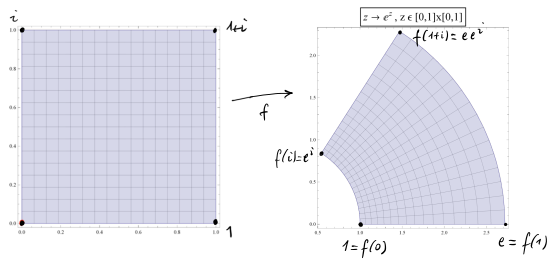
\includegraphics[width=0.6\linewidth]{images/analisi_complessa/es_mappa_conforme4.png}
        \caption{Visualizzazione della mappa $e^z$ conforme su tutto $\C$}
        \label{fig:mappe_conformi_esempio3}
      \end{figure}
    \item Sia invece
      \begin{equation*}
        f(z) = \frac{z^2 - i}{z^2 + i} 
      \end{equation*}
      questa risulta essere conforme su 
      \begin{equation*}
        \C \setminus \left\{ 0, \frac{\sqrt{2}}{2} - \frac{\sqrt{2}}{2}i,
        -\frac{\sqrt{2}}{2} + \frac{\sqrt{2}}{2}i \right\}
      \end{equation*}
      In particolare è conforme su tutto il primo e terzo quadrante.

      \begin{figure}[h]
        \centering
        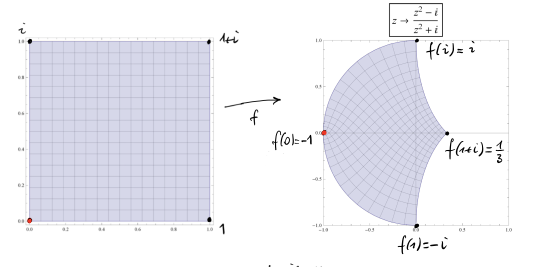
\includegraphics[width=0.6\linewidth]{images/analisi_complessa/es_mappa_conforme5.png}
        \caption{Visualizzazione di $f$ sul primo quadrante}
        \label{fig:mappe_conformi_esempio4}
      \end{figure}
  \end{enumerate}
\end{example}
